%
% 
%
%

\chapter{Classification of Dynamic Tracing Techniques}
\label{sec:Classification}
In contrast to static tracing, dynamic tracing is based on the idea of allowing
trace collection of running programs and unmodified binaries. Any necessary
steps to enable such collection is therefore performed at runtime.

Given this rather broad definition of dynamic tracing, a variety of approaches for
implementing dynamic tracing can be identified by studying existing research papers
and implementations. The individual concepts and algorithms encountered among these 
approaches vary, yet a small number of key ideas shared among groups of
approaches can be identified. Based on this insight, this section proposes a classification of 
dynamic tracing techniques.

Although the focus of the remaining discussion lies on kernel mode instrumentation, user
mode instrumentation solutions are discussed as well. Moreover, approaches targeting
broader application than just tracing -- such as profiling or dynamic optimization --
are discussed for sharing many properties with dynamic tracing approaches.
Virtualization-based approaches, however, in which the entire operating system 
is run in a virtual environment are considered out of the scope of this work.
%
%Tracing can be performed on various levels of detail -- i.e. the amount of code
%a single trace output corresponds to differs sharply. If, for example, system
%call invocations are traced, a single trace output (e.g NtCreateProcess has been
%called) may signalize immense amounts of code to be about to be executed.
%
%On the other hand, tracing can be performed on a very fine grained level -- 
%an example for this is instruction-level tracing, which some tracing solutions
%support.
%
%In the context of this work, tracing on the level of routine calls is of primary 
%interest. All techniques and solutions discussed in the
%following section support at least this level of detail, although some also allow
%more fine grained information to be captured.


Any tracing solution, regardless of the level of detail supported, 
relies on the consumption of events, although the nature of the
individual events of interest may vary. However, a first rough distinction of techniques can
be made based on the source of these events, which is either hardware or software. 
%Approaches
%based on software can be further broken down, as illustrated by the following diagram. 

Each of the classes will be discussed individually in the following sections. Along with
this discussion, a non-exhaustive list of solutions implementing the individual technique
is presented.

\begin{figure}[htbp] 
\begin{centering} 
%  (x, y), (x, y) from lower left corner
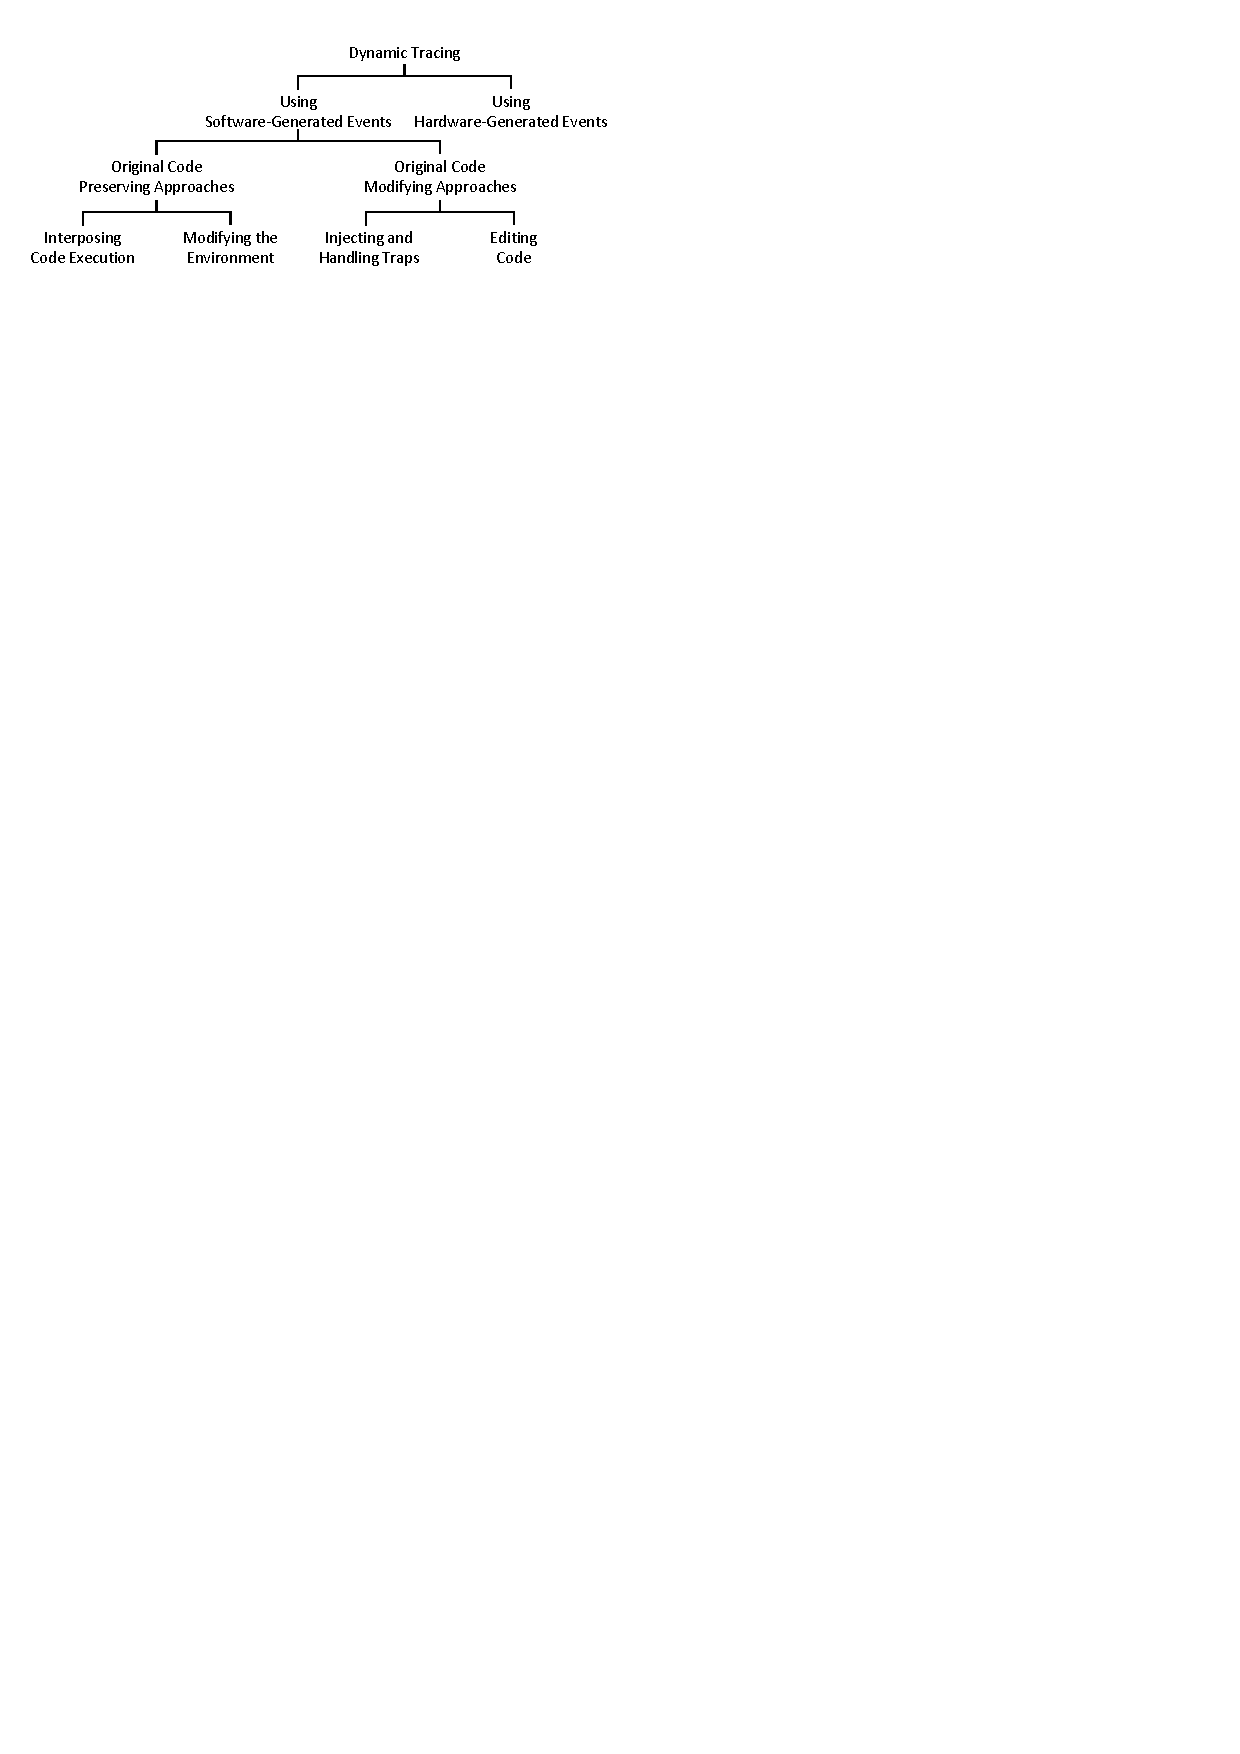
\includegraphics[scale=1.3, clip=true, viewport=0cm 25cm 11cm 30cm]{images/diagrams/Classification.pdf} 
\caption{Classification of Dynamic Tracing Techniques} 
\label{Classification} 
\end{centering} 
\end{figure}

It is worth pointing out that the classification refers to \emph{techniques} rather than
solutions. Although the majority of tools and solutions leverages a single 
such tracing technique only, there are solutions that combine two or more 
of the presented techniques.

% degree of granularity --> function level of prim interest

% clas virt/non-virt?
% Alt: probe-based [olszewski], non probe-based?

\section{Using Hardware-Generated Events}
\subsection*{Definition} 
A tracing technique that utilizes events generated by the CPU while executing unmodified code.

\subsection*{Discussion}
Current processors such as those of the IA-32 family offer features for generating and
recording a number of performance and tracing-related events. Although current IA-32 processors do 
not offer a means to specifically record subroutine calls, they do allow the generation and recording
of more fine grained events. A notable feature in this context is \emph{last branch recording} 
\cite{intel07_3B}, which records origin and target of the last branches taken. Using this and 
similar processor features, a tracing solution could also deduce more coarse-grained 
tracing information such as procedure-level traces.

As the collection of tracing information is based on dedicated hardware features, 
no code has to be modified. In particular, although this technique may require handling of 
traps, the code does not need to be augmented by trap-generating instructions. 

\subsection*{Implementations}
The facilities provided by CPUs that may be used for observing execution flow
tend to generate very fine-grained information, often on an instruction or 
branch-level basis. Moreover, features such as last branch recording are rather new additions 
to the IA-32 instruction set and cannot be expected to be widely supported yet. 
Still, solutions for procedure-level execution analysis
can be identified to rely on such events, although their number seems to be limited.

One of the most common tools that rely on hardware events are sampling profilers. However, the 
use of sampling to obtain tracing and performance information is arguable due 
to the inherent risk of impreciseness -- a topic that has been discussed extensively in 
\cite{Tamches01}. Yet, these tools rely on frequent timer
interrupts, which are clearly events generated by hardware rather than induced by software. In
the context of the NT kernel, a notable example of a facility that uses sampling is
the built in profiling facility \cite{Nebbett00}, which serves as the basis for the kernrate tool.

% VTune http://developer.intel.com/vtune/analyzer/index.htm.

Linux kernel version 2.6.25, which was in the state of a release candidate at the time of 
writing, introduces an enhancement for \emph{ptrace} which makes use of branch 
trace storage \cite{intel07_3B} on IA-32 processors \cite{Molnar08}. 


% more?
% http://www.openrce.org/blog/view/535/Branch_Tracing_with_Intel_MSR_Registers
% http://kerneltrap.org/Linux/x86_Architecture_Changes_Merging_in_2.6.25
% http://kerneltrap.org/mailarchive/linux-kernel/2008/1/21/588524



\section{Using Software-Generated Events}
\subsection*{Definition} 
A tracing technique that utilizes events caused by software. As unmodified 
code is assumed not to generate the necessary events, adaptions to the code
or the way the code is executed is usually required.

\subsection*{Discussion}
To allow a more precise discussion of the ideas behind this class of tracing techniques, this class is further 
broken down into \emph{Original Code Preserving Approaches}
and \emph{Original Code Modifying Approaches}. These classes will be discussed
separately.






\section{Original Code Preserving Approaches}
\subsection*{Definition}
A tracing technique that causes the generation of events necessary for the collection of 
tracing information without performing in-place modifications on 
the original code. 

\subsection*{Discussion}
In order to provoke the generation of such events without modifying affected
code, two approaches can be taken. On the one hand, the execution flow of the
code can be adapted by changing its environment, e.g. by performing changes
on data. On the other hand, different code may be executed, which may
or may not be derived from the original code.

The following two sections discuss both approaches.


%\section{Solutions Relying on Environment Modification}
\section{Modifying the Environment}
\label{sec:EnvMod}
\subsection*{Definition}
A tracing technique that does not rely on modifying code but rather on altering
the environment the code is executed in with the intent 
of adapting the behavior of the software in
a manner that allows tracing information to be gathered.


\subsection*{Discussion}
The most prominent example of modifications on the environment that affect execution flow is 
exchanging the values of memory locations storing addresses used for indirect calls. 
By altering these locations, a branch into tracing code may be injected which,
besides collecting the desired information, delegates to the original target. Figure
\ref{IndirectCalls_Thunked} illustrates this idea.

\begin{figure}[htbp] 
\begin{centering} 
%  (x, y), (x, y) from lower left corner
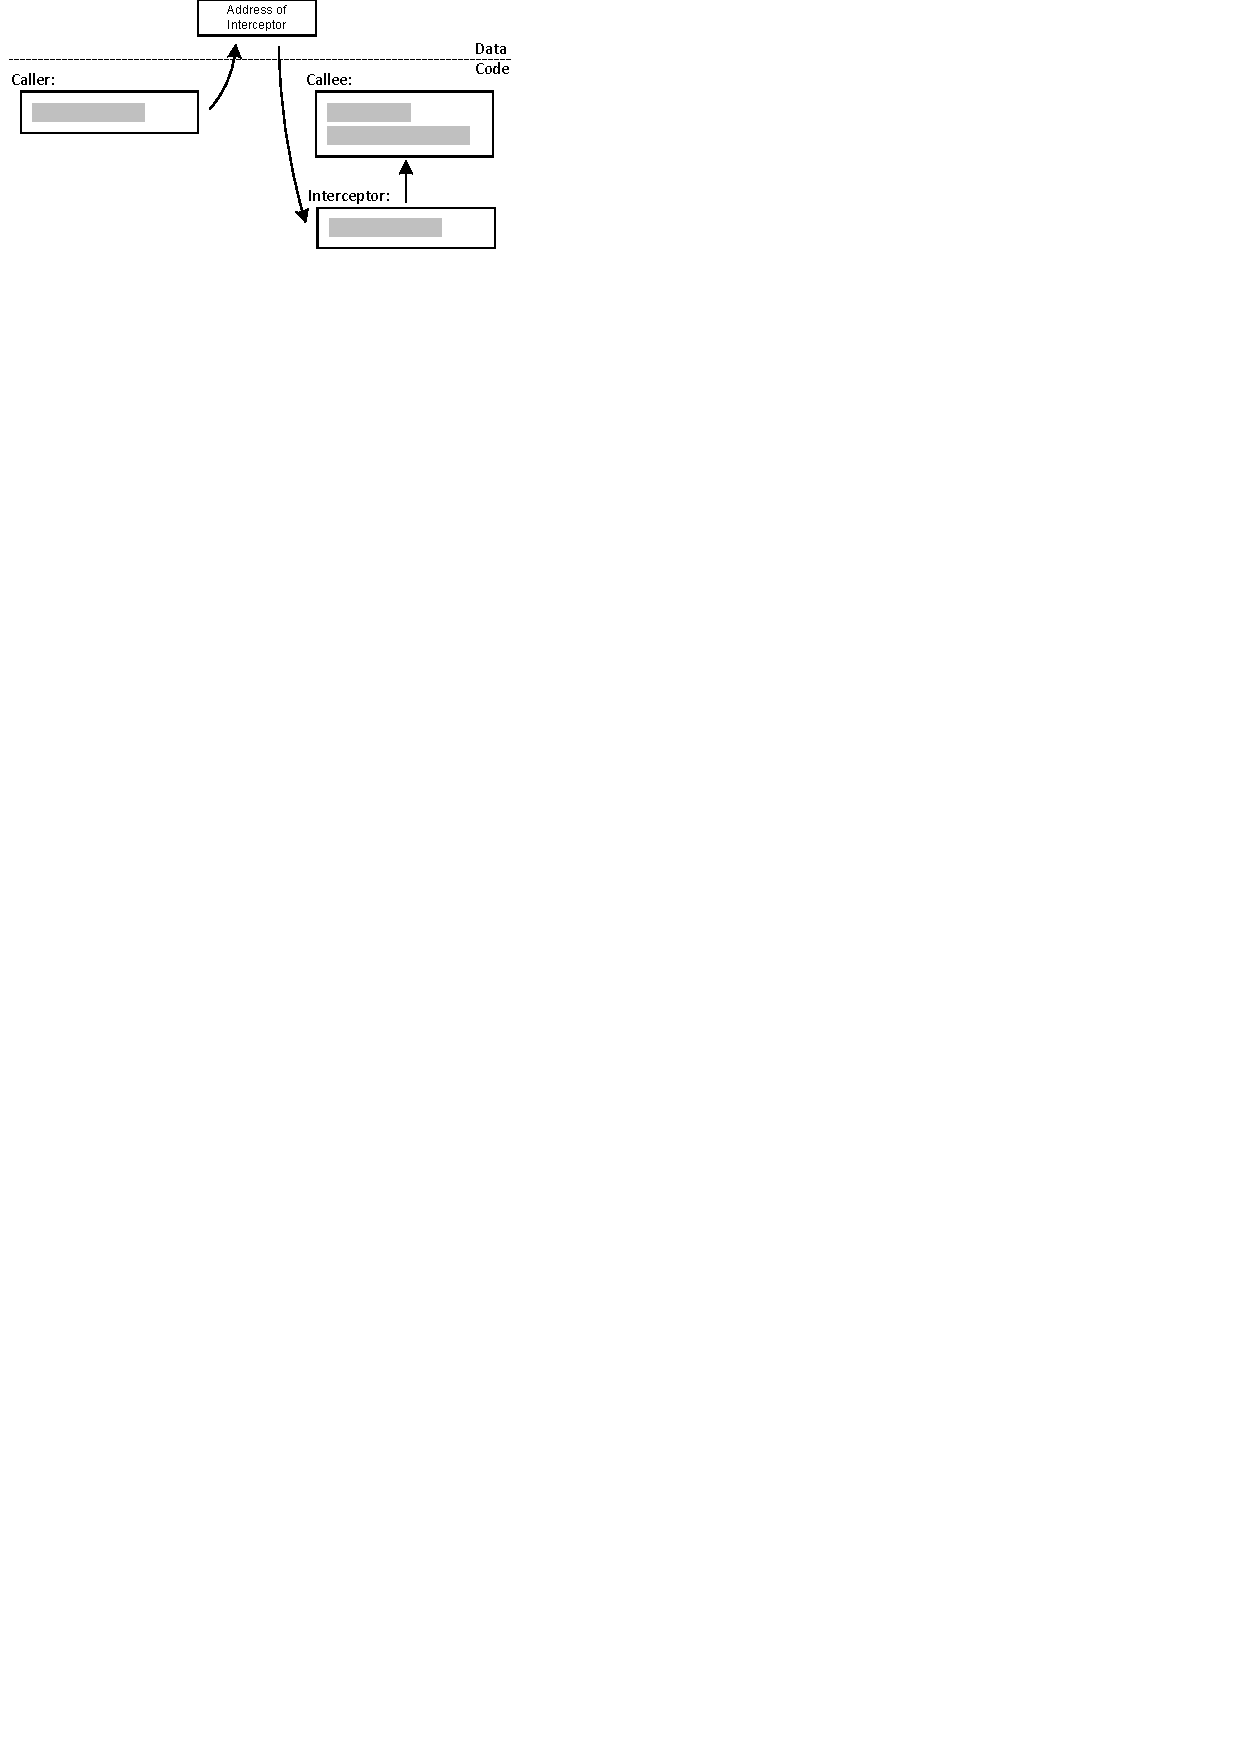
\includegraphics[scale=1, clip=true, viewport=0cm 25cm 9cm 30cm]{images/diagrams/IndirectCalls_Thunked.pdf} 
\caption{Intercepting an indirect call} 
\label{IndirectCalls_Thunked} 
\end{centering} 
\end{figure}

%This practice of call interception has been brought up before as an alternative
%to caller- or callee-site tracing. As only the memory locations storing target
%addresses used for the indirect branches need to be modified, both caller and
%callee routines may remain untouched. However, interception
%of all potential calls to a specific routine may not be feasible using
%this approach as only calls from specific origins can be intercepted and traced.

Whether this approach is applicable or not significantly depends on the individual
software to be inspected. Code that does not make use of indirect jumps
or whose execution flow cannot be adapted by data modifications in a sufficient manner
may not be traceable with such an approach. In contrast, a piece of software may explicitly
have been designed for allowing this kind of observation. Such software
may, for example, make extensive use of \emph{jump tables}. 

The majority of software may be expected
to fall in between these two extremes -- these systems have not been explicitly
designed for allowing tracing but for other reasons make use of programming techniques
that can be leveraged for this intent. Examples for such techniques 
include \emph{Vtables} as used by C++, COM \cite{Box98} and other object oriented languages and
frameworks. Jump tables are very similar to Vtables in that they also store function 
pointers, although they are usually unrelated to the concepts of object orientation. 

A prominent
example for a jump table is the \emph{Import Address Table} (IAT) defined by the 
\emph{Portable Executable File Format} \cite{Pecoff06}. The role of the IAT is to serve
as the connector between dynamically loaded modules. Whenever a module such as a DLL
imports routines from different modules, its IAT will provide one slot for each import.
When the respective module is loaded, the loader will resolve these imports and will 
store the pointers to the imported routines in the corresponding slots of the IAT. 

The \emph{Procedure Linkage Table} (PLT) defined by the \emph{Executable and Linking Format} (ELF) \cite{elf}
employs a similar mechanism. Like the IAT, the PLT is used to allow function calls to be made 
from one executable or shared object to another.

Without restricting this discussion to a specific software package that is to be 
instrumented, the general applicability of such approaches is therefore hard to 
quantify, but can at least be expected to be significantly below approaches relying on code
modification.


\subsection*{Implementations}
The NT kernel makes extensive use of function pointers. While most of these can
be expected not to be designed for the purpose of intercepting or tracing operations,
some of them are. A prominent example of such \emph{hooks} are those used by
Driver Verifier \cite{DriverVerifier}.

Microsoft Driver Verifier is a tool for detecting common flaws in drivers. To detect
certain erroneous operations, Driver Verifier has to observe a driver on a rather
fine grained level. Among the techniques used by Driver Verifier to attain this 
observation is to intercept a number of routine calls. For this purpose, the NT kernel 
deliberately uses function pointers at certain places with the intent of enabling 
Driver Verifier to hook into calls. An example for such an operation
is calling a driver, as implemented by \verb|IofCallDriver|.

As listing \ref{IofCallDriver} suggests, the global variable \verb|pIofCallDriver| is NULL
during normal operation. To allow hooking, the variable can be set to 
point to a routine such as \verb|IovCallDriver| (part of Driver Verifier).
Besides pre- or postprocessing the call, such a routine will usually 
delegate the call to \verb|IopfCallDriver|.


\begin{lstlisting}[label={IofCallDriver}, caption={Implementation of IofCallDriver, WRK 1.2, \\ BASE$\backslash$NTOS$\backslash$IO$\backslash$IOMGR$\backslash$iosubs.c, line 2237}]
NTSTATUS
FASTCALL
IofCallDriver(
    IN PDEVICE_OBJECT DeviceObject,
    IN OUT PIRP Irp
    )
{
  if (pIofCallDriver != NULL) {

    //
    // This routine will either jump immediately to  
    // IovCallDriver or IoPerfCallDriver.
    //
    return pIofCallDriver(
	    DeviceObject, Irp, _ReturnAddress());
  }

  return IopfCallDriver(DeviceObject, Irp);
}
\end{lstlisting}

%stacktraces


As empirical analysis reveals, \emph{IRPTracker} \cite{NtInsider03}, a tool that allows
tracking of \emph{I/O Request Packets} (IRPs) traveling through the I/O subsystem, also leverages this (undocumented)
facility to gather tracing information.

%If routine calls are to be traced at module boundaries, another tracing option 
%is to leverage the loader. When the loader is about to load a module, it will search
%for the respective file in a number of directories. This behavior can be exploited by
%placing a specially crafted module in a directory being searched before the directory
%the actual module is located in. This module has to provide the same interface, i.e.
%the same set of exports. Whenever one of these routines is invoked, it can trace the call.
%Yet, in order to provide the same functionality as the original module, it further has
%to delegate each call to the corresponding routine of the original module. For this purpose,
%the tracing module has to explicitly load the original module

Another common technique used for intercepting routine calls -- either to adapt behavior or
to implement tracing -- is \emph{Import Address Table Hooking} \cite{Robbins03}. 
By replacing a function pointer in the IAT with a pointer to an appropriate tracing
routine, inter-module calls can be traced. However, any calls not crossing a module 
boundary or using function pointers obtained dynamically (such as by using \verb|GetProcAddress|) cannot be 
easily intercepted with IAT hooks. Notwithstanding these limitations, 
applied to core OS libraries such as ntdll.dll or
kernel32.dll, IAT hooks are a powerful technique for observing the interaction between 
a user mode program and the operating system. As demonstrated by Leman \cite{Leman00}, this
approach is not only applicable in user mode but also in kernel mode. 

Clowes \cite{injectso} has shown that a similar technique can be employed to leverage the
ELF PLT in order to intercept function calls.

A related, yet more specialized technique is hooking the \emph{System Service Descriptor Table}
of the NT kernel, as first published in \cite{Russinovich97}. In a similar manner, calls to
interrupt service routines can be intercepted and delegated \citep{Hoglund05, UndocNT}. 
However, these techniques belong to the practices explicitly 
discouraged by Microsoft \cite{Microsoft07}. More
kernel mode function pointer-based techniques have been discussed in the context of 
security research in \cite{Skywing07}.

The \emph{COM Universal Delegator} \citep{Brown99_1, Brown99_2} defines a 
method call interception framework for the \emph{Component Object Model} (COM). 
The basic idea behind this approach is to leverage the fact that all
methods of a COM interface are virtual and method invocations are dispatched through a 
Vtable. In order to intercept all method invocations of a respective interface, the 
pointers to the methods stored in the Vtable are replaced by pointers to specific \emph{thunk} 
routines. After preprocessing a call, a thunk routine will remove itself from the stack
and delegate the call to the original method implementation. Using return address replacement
and a thread local private stack, the framework is also capable of additionally intercepting
method returns in order to post-process a call.

A similar approach that additionally allows cross-process tracing of COM method invocations 
has been published in \cite{Leman99}.

As published, both approaches only apply to COM and user mode. However, the basic idea of 
implementing virtual method dispatching by using Vtables is equally applied in other 
programming environments. Therefore, this approach could be adapted to be applicable to
other scenarios and environments, including kernel mode Windows, as well. 
% VC++?

%Although the framework makes use of services available in user mode exclusively (such as 
%thread local storage), leveraging the basic ideas of the Universal Delegator 
%in kernel mode seems to be viable. As discussed, the technique relies on Vtables, which,
%as the predominant language used for kernel development is C, can be expected not to
%be encountered frequently in the kernel. However, the technique can be applied in 
%a similar manner to jump tables and other indirect calls. As such, the 
%basic ideas can be expected to be of significance in kernel mode as well
%

% simulation?
\section{Interposing Code Execution}
%\section{Solutions Relying on Code Interposition}
\subsection*{Definition}
A tracing technique that relies on interposing the code to be traced. Rather than 
letting the affected regions of original code run natively, code is treated 
as data and used as information for interpreting or derivation of new code.

\subsection*{Discussion}
The basic idea behind these solutions resembles virtual machines in that
they rely on techniques such as interpreting code or using \emph{just in time compilation} 
techniques to derive new code from the original code. In 
both cases, the software gains the option to intercept certain operations or
to augment the code by instrumentation code on the fly. 

The latter technique, fetching original code fragments, augmenting it and assembling new code 
fragments is commonly referred to as \emph{dynamic compilation} \cite{cmelik94shade}. 
The resulting code fragments, called \emph{translations}, are encoded using the same instruction
set as the original code. This differs from \emph{dynamic binary translation} \cite{cifuentesbinary},
which describes a similar technique, yet involves translating between different instruction 
sets. 

Dynamic compilation offers immense flexibility with regard to the level of
detail at which instrumentation can be performed. With regard to function
boundary tracing, this flexibility allows the user of such a solution to make a very specific
choice of how a routine call should be traced. On the one hand, the event of 
\emph{calling} a routine could be captured by identifying and instrumenting all code
sequences that call the respective routine. On the other hand, the tracing could be
performed at the callee's site, i.e. the event of a routine \emph{being called} could be captured
by instrumenting the respective routine itself.

Both of these options have their own advantages and disadvantages.
On the one hand, as there is usually more than one potential caller of a given 
routine, tracing on the caller's site offers the ability to further distinguish
between calls. For instance, by instrumenting specific callers only, tracing
can be scoped to affect only those routine calls performed from 
specific locations in code. On the other hand, when all calls are to be captured --
regardless of their origin -- a potentially large number of calls must be properly
instrumented. In contrast to that, callee-site instrumentation only requires
the routine itself to be instrumented and guarantees all calls to be captured.

In practice, however, caller-site tracing is often limited by the fact that determining all
potential callers of a given routine is challenging due to the existence
of indirect jumps and calls. 


%In contrast to many virtual machinee implemetations which operate 
%on \emph{byte code} optimized for the consumption by virtual machines however, 
%dynamic compilation solutions have to operate on IA-32 machine code. Due to the 
%relative complexity of this instructions set, solutions of this class tend to 
%be significantly more complex than solutions
%of other classes.


\subsection*{Implementation}

\emph{Shade} \cite{cmelik94shade} was among the first tools to implement dynamic compilation. 
Rather than being launched directly, an application that is to be instrumented is run
via Shade. That is, a user launches Shade and requests it to load the respective 
binary. Although this approach prohibits attaching to a natively running process after
the fact, it gives Shade tight control over the execution of the target. Shade
uses this control to avoid all execution of native, unmodified code. Instead, 
Shade makes extensive use of dynamic compilation and only executes the 
dynamically compiled, instrumented code.

As part of this dynamic compilation, Shade allows calls to \emph{trace functions} 
to be injected before certain instructions. Using such callbacks, tools such as 
call profilers and call graph analyzers can be built on top of Shade.

By using appropriate caching mechanisms, Shade aims at compensating the additional 
overhead of instrumentation and attains reasonable performance. Shade allows instrumentation
of user mode SPARC binaries and has been implemented for Solaris.

\emph{Dynamo} \cite{Dynamo00} focuses on dynamic optimization -- its aim is to transparently 
improve execution speed of just-in-time generated or even statically optimized 
code. The basic strategy of Dynamo is to start off as a machine code interpreter. 
Observing program behavior, Dynamo is capable of identifying \emph{hot}, 
i.e. frequently executed code regions, which it will attempt to optimize. 
Acting on the level of \emph{traces}, i.e. sequences of consecutively executed instructions, 
Dynamo makes use of dynamic compilation facilities similar to Shade to create optimized 
versions of these traces, so called \emph{fragments}. To account for the frequent use of 
these code regions, these fragments are cached.

Dynamo has been implemented as a shared library for the PA-8000 architecture 
and allows being attached to a running process. Although the 
approach would allow further instrumentation for purposes such as tracing,
Dynamo does not offer such facilities by itself. Still, Dynamo has delivered the groundwork
for DynamoRIO, which allows both optimization and instrumentation of applications.

\emph{DynamoRIO} \cite{Bruening04} is a dynamic code manipulation solution
for user mode applications on Linux and Windows. DynamoRIO allows runtime manipulation
of unmodified binaries for purposes such as tracing. DynamoRIO is similar
to Shade in that it also avoids execution of the original code altogether. The code is 
merely used as a blueprint for deriving, i.e. dynamically compiling, new code. Like
Shade, DynamoRIO also has to be loaded during process startup, i.e. before any
of the original code has become subject to execution. Attaching to an already running 
process is thus not possible.

As part of the compilation, code can be specified to be augmented 
by additional instrumentation code. Moreover, in order to improve execution speed, 
DynamoRIO is capable of applying certain optimizations to this code. Once compiled,
the code fragments are placed into a code cache, from which it can repeatedly be
fetched.

Based on this setup, DynamoRIO is able to dynamically instrument an application 
without the kernel or the application itself being aware of. DynamoRIO provides 
a rich set of interfaces that allow execution observation of the software on various levels, 
making it a system whose potential applications reach far beyond tracing on the
level of routine calls.

However, to attain this high degree of flexibility, DynamoRIO, like Shade, has to have 
tight control over the communication between the kernel and the process. Besides
system calls, this also includes interfaces such as user mode callbacks invoked 
by the kernel. While uncommon on Unix systems, such callbacks play an important 
role on Windows NT. Notwithstanding the complexity involved, DynamoRIO presents 
a solution that is capable of interposing all such interfaces in order not to lose
control over the process.


\emph{Valgrind} \cite{Nethercote04} is a user mode instrumentation 
framework for Linux/IA-32. It is designed to serve
as the foundation for analysis tools such as profilers and 
memory checkers. Technically, Valgrind translates the IA-32 machine 
code from the program to be run to an intermediate representation called 
\emph{UCode}, at which instrumentation is applied. The instrumented intermediate code 
is then translated back to IA-32 machine code which is finally executed. This instrumentation
is performed lazily on a basic block level.

Similar to Shade and DynamoRIO, Valgrind attempts to avoid the execution of original code. To
attain the necessary degree of control over code execution, Valgrind has to be 
attached during process startup as well. Like DynamoRIO, Valgrind interposes all major communication 
channels between the operating system kernel and the actual application code, including 
system calls and signal delivery.

Tools such as \emph{memcheck} and \emph{cachegrind} (part of the Valgrind Tools Suite \cite{ValgrindTools}) have 
shown the effectiveness and flexibility of Valgrind, which these tools are 
based on. The fact that Valgrind has to be loaded into the affected
process from the start is also of minor concern in the context of such tools. 

%Regarding the feasibility
%of porting Valgrind to Windows, the cited thesis states that "`because Windows has a completely
%different architecture to the aforementioned Unix-style operating systems, porting Valgrind to Windows
%would require extremely large changes"'. Moreover, given the degree of control both 
%DynamoRIO and Valgrind necessitate for their proper working, the feasibility of successfully 
%applying these approaches to kernel mode seems questionable.

Considering Valgrind, Shade and DynamoRIO for the purpose of dynamic instrumentation and tracing 
of running systems, however, the requirement of having to be loaded during process startup 
can turn out to be an issue. 

\emph{Pin} \cite{Pin05} is an instrumentation solution that shares several ideas with 
the aforementioned solutions. Pin allows instrumentation of user mode Linux and Windows processes and 
instruments code in a \emph{just in time} manner. Yet, unlike Shade, DynamoRIO and Valgrind, Pin is 
also capable of being attached to process after it has started and being detached without the
process having to be terminated.

While Pin is limited to user mode, Olszewski et al. \cite{Olszewski07} have brought the ideas of 
just in time instrumentation and late attachment to kernel mode. 
Sharing basic ideas with Pin, the presented solution 
allows instrumentation of kernel mode code on the Linux operating system.

Both approaches perform instrumentation by injecting additional
code sequences while leaving the original code unmodified: Basic blocks
are fetched from their original location, instrumented, compiled, and placed into a 
code cache as they become subject to execution. Whenever a new block is 
compiled, the branches from and to this block are updated. 
Any branches pointing to blocks not yet compiled are linked to 
a special \emph{dispatcher stub} which, when invoked, will trigger the 
just in time instrumentation of the respective block. 

Like the other solutions discussed in this section, Pin heavily 
relies on disassembly of the code to be instrumented 
in order to identify the basic blocks. 

However, having execution repeatedly branch between original code, dynamically
compiled code blocks, the dispatcher and instrumentation code 
presents an additional problem: The contents of certain registers may have to 
be preserved and later restored whenever such a branch is taken. 
One option is thus to save and restore all CPU registers in these situations,
which is guaranteed to be sufficient, yet, induces a non-negligible overhead. 
A more efficient, yet more challenging approach to implement is thus
to perform register liveness analysis -- a technique used by several solutions 
presented in this section, including Pin. By analyzing the usage of registers
beforehand, state saving can be limited to \emph{live} registers, i.e. registers
known to be referenced at a later stage.

Moreover, for any dynamic compilation technique that allows late attachment
to become effective, there 
has to be at least one point where control is initially transferred to 
the dispatcher of the instrumentation solution. Once having gained control, 
the dispatcher can then direct further instrumentation. To achieve
this initial takeover of control, these approaches therefore need some jump aid. Pin
uses the \emph{ptrace} infrastructure for this purpose while the solution proposed
by Olszewski et al. facilitates an additional instrumentation technique, namely using 
environment modification (see section \ref{sec:EnvMod}): it replaces entries of the system 
call table.

By writing the dynamically compiled code sequences to a new location and leaving
the original code untouched, the challenges and limitations of in place code 
modifications are largely avoided. An implication of this approach, however,
is that the process maintains up to two copies of each block -- 
the dynamically compiled, and the original code block. Disregarding the increased 
memory requirements, this coexistence of instrumented and uninstrumented 
code as well as the necessity for providing explicit entry points comes along with both 
notable advantages and disadvantages.

On the one hand, it may be advantageous that the instrumented piece of code 
(i.e. a sequence of instrumented basic blocks) is only executed when the execution flow originates
from a certain entry point, such as a system call. Tracing all memory allocations made by a specific 
system call may be an example for such a use case. Not only are memory allocations 
made by other system calls not traced, the overhead of instrumentation is also only
paid for those execution flows that are indeed of interest.

On the other hand, this scoping may well turn out to be a disadvantage. If, for example,
all memory allocations -- regardless of whether made in the context of a system call
or not -- are to be traced, such a solution can be inappropriate. More generally,
the effectiveness of the approach heavily depends on the area of interest,
(i.e. the code of which execution is to be traced), and the question whether it
can be fully covered by one or more of such entry points. 

Finally, solutions that do not support attachment to a running process do not 
fully qualify as being \emph{dynamic} in the sense expressed in the beginning
of this section. Those solutions that do allow late attachment usually require
some kind of bootstrapping. The applicability of such solutions 
is therefore also dependent on the flexibility of the \emph{jump aid} solution employed. 
The more entry points this solution allows, the greater the applicability 
of the solution will be. 

% SMP-safe






\section{Original Code Modifying Approaches}
\subsection*{Definition}
In order to generate the events necessary for tracing, in-place modifications 
on the previously unmodified, original code are performed. The code is 
augmented so that the necessary events are issued. Such events may include
traps or callback routines being invoked.

\subsection*{Discussion}
Instrumenting code requires augmenting the code by additional instructions -- instructions
that, for instance, capture tracing information. The basic problem all code modifying
solutions therefore have to face is how these additional instructions can be woven
into the original code. This question becomes even more relevant when instrumentation
is to be performed on a very fine grained level such as on the level of basic blocks
or instructions. 

\begin{figure}[htbp] 
\begin{centering} 
%  (x, y), (x, y) from lower left corner
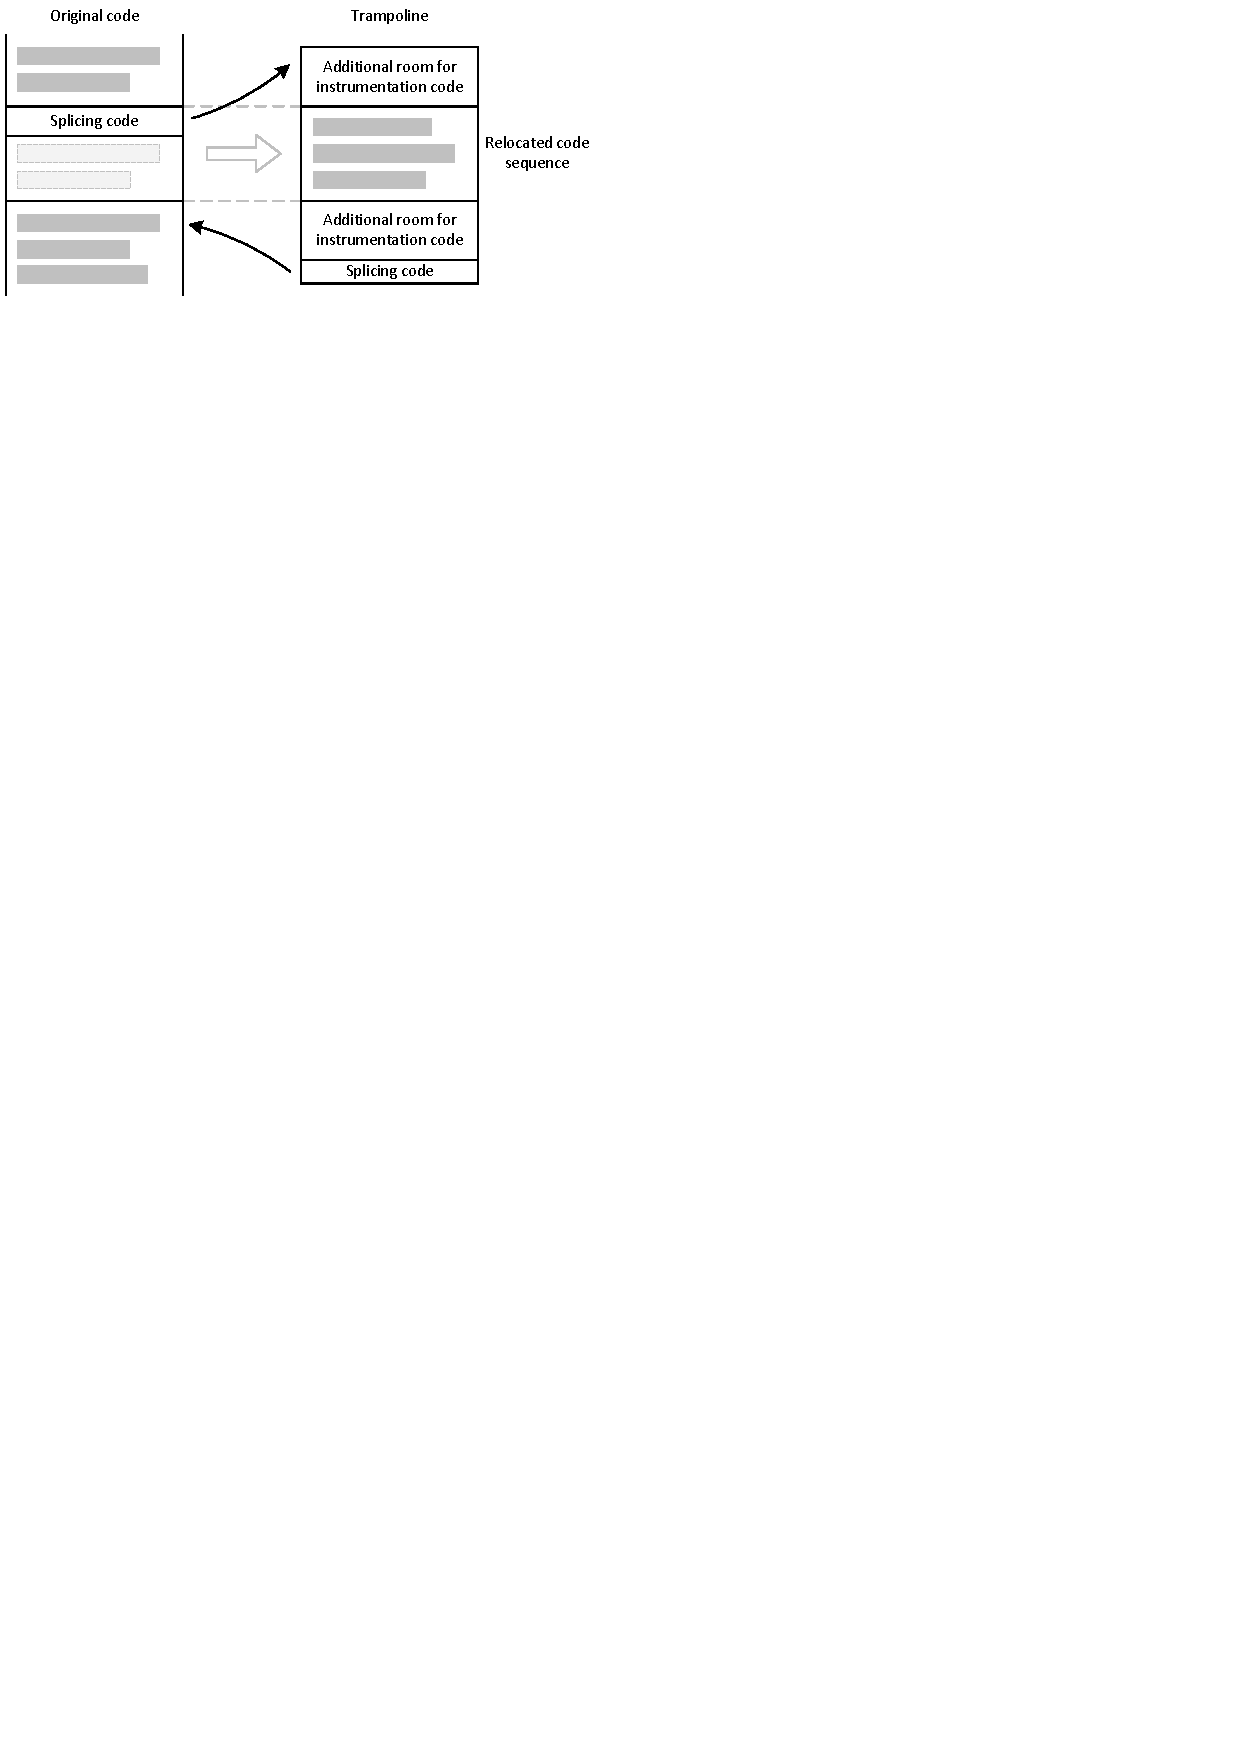
\includegraphics[scale=1, clip=true, viewport=0cm 24.5cm 10cm 30cm]{images/diagrams/CodeSplicing.pdf} 
\caption{Runtime code splicing} 
\label{CodeSplicing} 
\end{centering} 
\end{figure}

One pattern encountered in several solutions is \emph{runtime code splicing} \cite{thiemann99higherorder}. The idea
of runtime code splicing, illustrated in figure \ref{CodeSplicing}, is as follows: 
One or more instructions are \emph{cut} out of the original code. These instructions,
along with the necessary instrumentation code, are moved to a newly allocated code
block, usually referred to as \emph{trampoline}. The crucial point to notice is that the
trampoline usually is significantly larger than the piece of relocated code. 
The original code and this code block are then \emph{spliced} 
so that the execution flows from the original code to the trampoline and back to the 
remainder of the original code. Splicing can be applied on any level ranging from single
instructions (i.e. only a single instruction is relocated) to entire routines.
However, the relocation of code sequences has further ramifications such as the 
necessity to update all relative addresses used by the relocated instructions.

Especially in the context of runtime code splicing, the differences between
original code modifying techniques and code interposing techniques seem
to become blurred. The characteristic difference, however, can be found in the 
fact that the original code remains the scaffold for code splicing solutions:
significant parts of the code may have been relocated, yet, barring exceptions, 
execution flow is usually routed back to the original code at the end of each such
code block.

In contrast, the original code mostly loses its role as serving as the scaffold 
in the case of solutions implementing code interposition: the default is
that execution is not routed back to original code when the end of such a dynamically
allocated code block has been reached -- rather, execution is routed 
to the next dynamically compiled block. Execution being routed back to original 
code is an situation that either never occurs or can at least be considered a comparatively rare occurrence.

When used for tracing of routine calls, both caller-site and callee-site 
could be implemented using code modification. In practice, however, instrumenting at
the callee site is encountered significantly more often.

Regarding existing instrumentation solutions in more detail, it is notable that a significant number of 
solutions implementing code modification primarily rely on the use of trap-generating
instructions. Although many properties are shared among such trap-centric solutions and other, non trap-centric 
code modification solutions, a separation into two techniques is worth being made.

\section{Injecting and Handling Traps}
\subsection*{Definition}
A tracing technique that relies on in-place modification of the original code. 
In order to be able to interrupt, control, or trace execution, trap-generating instructions
are injected into the original code. Using an appropriate trap handler, the
events generated by such instructions can be handled accordingly. 

% Trap handler: distinguish betweeen events using HT etc?

\subsection*{Discussion}
Injecting trap-generating instructions like \verb|int 3| on IA-32 is the classical
approach taken by debuggers to implement breakpoints. As dealing with traps is at
the core of hardware and an operating system's capabilities, this approach can be expected to
be feasible on a very wide range of operating systems and hardware architectures. 

On variable-length instruction set architectures such as the the IA-32, relying on trap-generating 
instructions has the additional advantage that such instructions can be as short
as one byte. With such short instructions, several of the challenges concerning runtime
code modification can be circumvented -- a topic that will be discussed in more detail 
in section \ref{sec:ChallengesOfRuntimeCodeModification}. 
A drawback of this approach, however, is the non-negligible overhead associated
with the handling of traps.


% -> Debugger Implementation
% placing 0xccs
% can be used for code splicing

\subsection*{Implementations}
As mentioned before, debuggers are the most prominent example of tools using
this technique for implementing breakpoints. Current Windows debuggers such 
as WinDBG also offer tracing facilities, which make them relevant
in this discussion. However, as their name already suggests, \emph{breakpoint commands},
which are used for such tracing purposes, also rely on handling of
debug traps.

%as gdb and WinDBG also offer tracing facilities, which makes them relevant
%in this discussion. Both \emph{tracepoints} as offered by gdb and WinDBG 
%\emph{breakpoints commands} are in fact implemented based on this technique. 

% gdb tracpoints?!?


% wt, umss?
% ptrace?

Beyond the realm of debuggers, usage of this technique 
for tracing purposes can be found in \emph{Dynamic Trace},
a diagnostic facility introduced by OS/2 Warp 4 fixpack 4 \cite{Warp97}.
By injecting an \verb|int 3| instruction and handling the trap issued by
these instruction appropriately, the \verb|DosDynamicTrace| system call allows
intercepting procedure calls in device drivers or the kernel. Using expressions
formulated in a specialized language, this infrastructure along with the tool 
\emph{dtrace}\footnote{Distinguishable only by capitalization, this tool is entirely unrelated to \emph{DTrace}.}
allows calls as well as local variable contents to be captured and 
logged.

Inspired by Dynamic Trace, \emph{Dynamic Probes} (DProbes) implements the
same approach on Linux \cite{Moore01}. DProbes allows placing \emph{probepoints}
on arbitrary code locations in both kernel and user mode code. Like Dynamic
Trace, DProbes implements probepoints by injecting an \verb|int 3| 
instruction and handling traps appropriately. The replaced instruction
is later either single-stepped or emulated. DProbes has also adopted the 
idea of using a \emph{little language} for defining the actions to be taken whenever
a probepoint becomes active.

\emph{KernInst} \citep{tamches99finegrained,Tamches01} is a dynamic kernel instrumentation 
solution for Solaris and Linux that implements runtime code splicing. 
It has been designed and implemented to run on
unmodified kernels and can be loaded dynamically. Using splicing techniques, KernInst allows
very fine-grained instrumentation -- not only procedures and basic blocks,
but also individual instructions can be instrumented. 

On IA-32 hardware, KernInst uses injection of trap-generating instructions for 
implementing code splicing. Designed as a generic 
instrumentation solution, KernInst is capable of being used for several purposes, 
performance profiling and tracing being amongst them. 

\emph{DTrace} \cite{Cantrill04} is a dynamic instrumentation solution that has been originally developed 
for Solaris but has meanwhile been ported to other operating systems as well, including
Mac OS X and FreeBSD. Part of DTrace is the \emph{Function Boundary Tracing Provider},
which allows dynamic tracing of procedures. Like KernInst, the IA-32 implementation 
of DTrace relies on the injection of trap generating instructions. Instrumenting
a procedure works by replacing one of the first instructions of a procedure by a 
trap-generating instruction. For this to work, DTrace requires a procedure to begin 
with the common prolog \verb|push ebp; mov ebp, esp|. When the procedure is 
executed, DTrace will handle the trap and trace the event. In order to continue 
execution, the replaced instruction is emulated and control is transferred 
back to the remainder of the traced routine. In a similar 
manner, DTrace allows exit tracing by replacing \verb|ret|, \verb|leave| or \verb|pop ebp|
instructions with a trap-generating instruction and handling the trap appropriately. To allow such 
instrumentation, DTrace relies on information obtained from the disassembly of the routine.
Among the other features and providers offered by DTrace, it also defines a 
language for expressing the actions to be taken in case of a trace event.

% KProbes not limited to routines!?!
\emph{Kprobes} is a facility provided by the Linux kernel that allows hooking of kernel mode
code \cite{Mavinakayanahalli06} by using traps. As such, KProbes is not a tool in itself but rather serves as 
the basis for other debugging or monitoring tools such as \emph{Systemtap} \cite{Prasad05}. 
Kprobes is part of the Linux kernel 2.6 and, like DTrace, has been designed to work reliably both 
on single and multiprocessor systems.



\section{Editing Code}
\label{sec:EditingCode}
\subsection*{Definition}
A tracing technique that relies on in-place modification of the original code. To
intercept and trace execution at certain points, additional instrumentation code 
is incorporated into the original code.

In contrast to the technique of \emph{Injecting and Handling Traps}, in-place
modifications are not limited to injecting trap-generating instructions.

\subsection*{Discussion}
Incorporation of instrumentation code is mostly performed by injecting jumps
into the original code which divert execution to the instrumentation code and
finally back to the original code.

Although functionally similar to the idea of \emph{Injecting and Handling Traps},
the primary benefit of this approach is that jumps are significantly more lightweight
in terms of performance than the issuing and handling of a trap.

The downside of this technique, however, is the increased danger of 
runtime code modification-caused hazards -- a topic that will be discussed in
more detail in section \ref{sec:ChallengesOfRuntimeCodeModification}.

% tracing ISRs?
% overrun end of func


\subsection*{Implementations}
The variable-length instruction set of the IA-32 architecture leads to several 
complications regarding code editing. On the one hand, disassembly requires 
significantly more attention than on a fixed-length instruction set architecture. 
This issue is discussed in more detail in section \ref{sec:Disassembly}. 

On the other hand, the IA-32 instruction set includes instructions as short as
one byte. Instrumenting code sequences including such single byte instructions by 
injecting a jump instruction may turn out to problematic. The shortest jump 
instruction offered by this architecture occupies two bytes and may thus lead
to requiring more than one instruction to be replaced. However, as will be discussed
in more detail in section \ref{sec:PreemptionAndInterruption}, such practice
can lead to issues with respect to concurrency and preemption.

Solutions such as KernInst and DTrace circumvent these challenges by reverting to
trap-based solutions on the IA-32 architecture. On SPARC, however, which is a
fixed length instruction set architecture \cite{SparcP07}, 
both KernInst and DTrace rely on embedding jump instructions into existing
code. In order to allow safe runtime instrumentation, 
in-place code modifications are restricted to comprising a single 
instruction only. KernInst uses these jumps to splice basic blocks while DTrace uses the jumps to
direct execution flow to trampolines, which in turn transfer control into 
DTrace \cite{Cantrill04}.

\emph{Paradyn} \cite{hollingsworth94dynamic} is an early 
implementation of an instrumentation solution that uses code editing in conjunction with runtime code splicing.
Targeted at collecting fine-grained performance measurements for parallel applications,
Paradyn injects calls to trampolines\footnote{Paradyn uses two types of trampolines,
base trampolines and mini trampolines. However, the differences between these types
of trampolines are irrelevant to this discussion.} into the original code. To clear
space for placing jumps to these trampolines, Paradyn relocates one or more instructions
to the trampoline. Once execution flow has reached the trampoline, these relocated
instructions along with the respective instrumentation code is executed, before
execution is redirected back to the remainder of the original code. Moreover, 
Paradyn allows being attached to a running process.

% RISC, but x86 available as well. No authorative information on this topic found.

Built on top of Paradyn, \emph{Dyninst} \cite{Dyninst00} provides a framework and an object
oriented API for controlling and instrumenting processes.


\emph{GILK} \citep{Pearce00,Pearce02} is an instrumentation tool for the Linux kernel. Similar to KernInst,
GILK implements runtime code splicing and allows instrumentation on basic block
level. Unlike KernInst, however, GILK uses jumps rather than trap handling 
techniques to divert execution flow on IA-32 systems. As will be discussed in section 
\ref{sec:PreemptionAndInterruption}, GILK only works on non-preemptable Linux 
kernels and does, in its current state, not support SMP systems.

Another implementation of code editing on IA-32 is \emph{Detours} \cite{Brubacher99}. 
Although limited to user mode code, Detours is noteworthy for providing 
a lightweight, yet widely applicable solution that poses only little 
requirements on the code to be instrumented. Detours can be used to either
redirect execution to an alternative implementation of a routine or to intercept
function entry. In both cases, Detours replaces one or more instructions located
at the very beginning of a function in 
order to preprocess or redirect a call. The replaced instructions are moved 
to a \emph{trampoline}, which, after preprocessing has been finished, is 
used to resume execution. Potentially replacing multiple instructions, Detours 
is, however, exposed to a number of issues that are discussed in 
section \ref{sec:SafetyConcerns}.

\emph{Vulcan} \cite{Vulcan01} is similar to GILK in that it also implements runtime code 
splicing. Although Vulcan is limited to user mode Windows, it stands out
by the fact that it allies static and dynamic instrumentation techniques
for a number of different architectures (IA-32, IA-64, MSIL) in a single 
tool.

\emph{Djprobe} \cite{Hiramatsu07} is an enhancement of Kprobes that uses 
jumps rather than traps to instrument routines. In comparison to Kprobes,
the applicability of djprobe is slightly more restricted. Yet, due to the
usage of jumps rather than traps, djprobe performs significantly better
than Kprobes \cite{Djprobes05perf}, which is also the main motivation behind this approach.
% optional ref: http://lkst.sourceforge.net/docs/probes-eval-report.pdf 

Djprobe is also noteworthy for thoroughly addressing safety issues related
to multiple instruction modification and patching of potentially non-quiescent code.
A key aspect of their algorithm for preventing preemption-related hazards
is to rely on \verb|freeze_processes|. This routine, which is primarily used
for system suspension, puts all user mode processes as well as all kernel
threads that have registered as being \emph{freezable} effectively to sleep \cite{Wysocki08}.
However, the paper does not discuss the safety of this approach 
in the existence of non-freezable kernel threads, i.e. threads that have
not registered as being freezable but may still be affected by certain
code patches.

